\documentclass[9pt,landscape]{memoir}
\usepackage{multicol}
\usepackage{calc}
\usepackage{ifthen}
\usepackage[landscape]{geometry}
\usepackage{hyperref,siunitx}
\usepackage{amssymb,amsmath,verbatim,graphicx,enumitem,microtype,upquote,units,booktabs,siunitx,hyperref}

\ifthenelse{\lengthtest { \paperwidth = 11in}}
{ \geometry{top=.5in,left=.5in,right=.5in,bottom=.5in} }
{\ifthenelse{ \lengthtest{ \paperwidth = 297mm}}
    {\geometry{top=1cm,left=1cm,right=1cm,bottom=1cm} }
    {\geometry{top=1cm,left=1cm,right=1cm,bottom=1cm} }
}

% Turn off header and footer
\pagestyle{empty}
\renewcommand{\familydefault}{\sfdefault}
\setlist[itemize]{leftmargin=0pt, noitemsep, before={\vspace*{-.25\baselineskip}}, after={\vspace*{-\baselineskip}}}
\setlist[enumerate]{leftmargin=0pt, noitemsep, before={\vspace*{-.25\baselineskip}}, after={\vspace*{-\baselineskip}}}

% Redefine section commands to use less space
\makeatletter
\renewcommand{\section}{\@startsection{section}{1}{0mm}%
    {-1ex plus -.5ex minus -.2ex}%
    {0.5ex plus .2ex}%x
{\normalfont\large\bfseries}}
\renewcommand{\subsection}{\@startsection{subsection}{2}{0mm}%
    {-1explus -.5ex minus -.2ex}%
    {0.5ex plus .2ex}%
{\normalfont\normalsize\bfseries}}
\renewcommand{\subsubsection}{\@startsection{subsubsection}{3}{0mm}%
    {-1ex plus -.5ex minus -.2ex}%
    {1ex plus .2ex}%
{\normalfont\small\bfseries}}
\makeatother

% Define BibTeX command
\def\BibTeX{{\rm B\kern-.05em{\sc i\kern-.025em b}\kern-.08em
T\kern-.1667em\lower.7ex\hbox{E}\kern-.125emX}}

% Don't print section numbers
\setcounter{secnumdepth}{0}


\setlength{\parindent}{0pt}
\setlength{\parskip}{0pt plus 0.5ex}

\makeatletter
\newsavebox\myboxA
\newsavebox\myboxB
\newlength\mylenA

\newcommand*\xoverline[2][0.75]{%
    \sbox{\myboxA}{$\m@th#2$}%
    \setbox\myboxB\null% Phantom box
    \ht\myboxB=\ht\myboxA%
    \dp\myboxB=\dp\myboxA%
    \wd\myboxB=#1\wd\myboxA% Scale phantom
    \sbox\myboxB{$\m@th\overline{\copy\myboxB}$}%  Overlined phantom
    \setlength\mylenA{\the\wd\myboxA}%   calc width diff
    \addtolength\mylenA{-\the\wd\myboxB}%
    \ifdim\wd\myboxB<\wd\myboxA%
       \rlap{\hskip 0.5\mylenA\usebox\myboxB}{\usebox\myboxA}%
    \else
        \hskip -0.5\mylenA\rlap{\usebox\myboxA}{\hskip 0.5\mylenA\usebox\myboxB}%
    \fi}
\makeatother

\renewcommand{\hat}{\xoverline}

% -----------------------------------------------------------------------

\begin{document}

\raggedright
\footnotesize
\begin{multicols}{3}
    \section{One Factor Experiments}
    \begin{itemize}
        \item The different values of the factor are called the \textbf{levels} of the factor and cal also be called \textbf{treatments}.
        \item The objects upon which measurements are made are called \textbf{experimental units}.
        \item The units assigned to a given treatment are called \textbf{replicas}.
        \item There are $I$ \textbf{samples}, each from a different treatment.
        \item If particular treatments are chosen deliberately by the experimenter, rather than at random, then we say that it is a \textbf{fixed effects model}.
        \item We have $I$ samples each from a different treatment.
        \item The treatment means are denoted $\mu_1, \ldots, m_I$.
        \item The \textbf{sample sizes} are denoted $J_1, \ldots, J_I$. The total number in all samples combined is denoted $N$.
        \item The \textbf{hypothesis} that we wish to test is
            \begin{equation*}
                H_0 = \mu_1 = \ldots = \mu_1
            \end{equation*}

            versus

            \begin{equation*}
                H_1 = \text{two or more of the $\mu_i$ are different}
            \end{equation*}

        \item $X_{ij}$ denotes the $j$th observation in the $i$th sample.
        \item The variation of the sample means around the sample grand mean is measured by a quantity called the \textbf{treatment sum of squares} ($SSTr$)

            \begin{align*}
                SSTr &= \sum_{i = 1} ^I J_{i.} {(\bar{X}_{i.} - \bar{X}_{..})}^2 \\
                     &= \sum_{i = 1} ^I J_i \bar{X}_{i.}^2 - N \bar{X}_{..}^2
            \end{align*}

        \item The measure of the variation in the individual sample points around their respective sample means is called the \textbf{error sum of squares (SSE)}

            \begin{align*}
                SSE &= \sum_{i = 1} ^I \sum_{j = 1} ^{J_i} {(X_{ij} - \bar{X}_i)}^2 \\
                    &= \sum _{i = 1} ^I \sum _{j = 1} ^{J_i} X_{ij} ^2 - \sum _{i = 1} ^I J_i \bar{X}_i ^2
            \end{align*}

            The standard one-way ANOVE hypothesis test is valid \textit{under the following conditions}

            \begin{enumerate}
                \item The treatment population must be normal.
                \item The treatment populations must all have the same variance, denoted $\sigma ^2$.
            \end{enumerate}


            \vspace{2mm}
        \item The quantities $I - 1$ and $N - I$ are the \textbf{degrees of freedom} for $SSTr$ and $SSE$, respectively.

            \begin{equation*}
                MSTr = \frac{SSTr}{I - 1} \qquad MSE = \frac{SSE}{N - I}
            \end{equation*}

        \item It follows that

            \begin{align*}
                \mu_{MSTr} &= \sigma^2 \text{ when $H_0$ is true} \\
                \mu_{MSTr} &> \sigma^2 \text{ when $H_0$ is false} \\
                \mu_{MSE} &= \sigma^2 \text{ whether or not $H_0$ is true}
            \end{align*}

        \item When $H_0$ is true, $MSTr$ and $MSE$ have the same mean. Therefore, when $H_0$ is true, we would expect their quotient to be near $1$. The quotient is in fact the test statistic. The test statistic for testing $\mu_0: \mu_1 = \ldots = \mu_i$ is

            \begin{equation*}
                F = \frac{MSTr}{MSE}
            \end{equation*}

            When, $F$ tends to be near $1$. When $H_0$ is false, $MSTr$ is larger, and $F$ is greater than $1$.

        \item The analysis of variance identity is

            \begin{equation*}
                SST = SSTr + SSE
            \end{equation*}

            The actual equation is as follows:

            \begin{align*}
                SST &= \sum _{i = 1} ^I \sum_{j = 1} ^{J_i} {(X_{ij} - \bar{X}_{..})}^2  \\
                    &= \sum _{i = 1} ^I \sum_{j = 1} ^{J_i} X_{ij} ^2 - N\bar{X}^2
            \end{align*}

        \item Null hypothesis ($H_0$) assumed to be true. It is the ``status quo'' so we believe it unless there is sufficient evidence to reject it.
        \item Alternative hypothesis ($H_1$ or $H_\alpha$) hypothesis we want to establish, i.e. try to prove. It is ``against current thinking or status'' so strong evidence is needed to justify it is true.

        \item Decision rule (where $\alpha$ is the significant level):

            \begin{align*}
                p-\text{value} &< \alpha \implies \text{reject $H_0$} \\
                p-\text{value} &\geq \alpha \implies \text{fail to reject $H_0$}
            \end{align*}

        \item When equal numbers of units are assigned to each treatment, the design is said to be \textbf{balanced}.
    \end{itemize}


    \section{Two Factor Experiments}
    \begin{itemize}
        \item Notation for two-way ANOVA:

            \begin{description}
                \item[$I$] The number of levels of the row factor
                \item[$J$] The number of levels of the column factor
                \item[$I\times J$] The number of treatment combinations
                \item[$K$] The number of replicates for each treatment combination
                \item[$X_{ijk}$] The sample value for the $k$th replicate corresponding to the treatment combination formed by the $i$th level of the row factor and $j$th level of the column factor.
            \end{description}

        \item The two-way ANOVA model ($\mu$ is grand mean, $\alpha_i$ is the $i$th row effect, $\beta_j$ is the $j$th column effect, and $\epsilon$ is the error).

            \begin{align*}
                X_{ijk}        &= \mu + \alpha_i + \beta_j + \gamma_{ij} + \epsilon_{ijk} \\
                \alpha_i       &= \bar{\mu}_{i.} - \mu \\
                \beta_j        &= \bar{\mu}_{.j} - \mu \\
                \gamma_{ij}    &= \mu_{ij} - \bar{\mu}_i - \bar{\mu}_j + \mu \\
                \epsilon_{ijk} &= X_{ijk} - \mu_{ij}
            \end{align*}

        \item To test hypothesis for two-way ANOVA, test for the presence of interaction effects,

            \begin{align*}
                H_{0, AB}: \gamma_{11} = \gamma_{12} = \cdots = \gamma_{IJ} = 0 \\
                H_{H, AB}: \text{at least one of the $\gamma_{ij}$ is nonzero}
            \end{align*}

            Hypothesis for the main effects are tested \textbf{only if} the additive model holds \textit{i.e., we fail to reject $H_{0, AB}$ for the first hypothesis test}. If interaction effects \textbf{does not exist}, continue to test the main effects.

            Test the main effects of the row factor $(A)$,

            \begin{align*}
                H_{0, A}: \alpha_1 = \alpha_2 = \cdots = \alpha_I = 0 \\
                H_{1, A}: \text{at least one of the $\alpha_i$ is nonzero}
            \end{align*}

            The main effects of the column factor is the same.
    \end{itemize}

    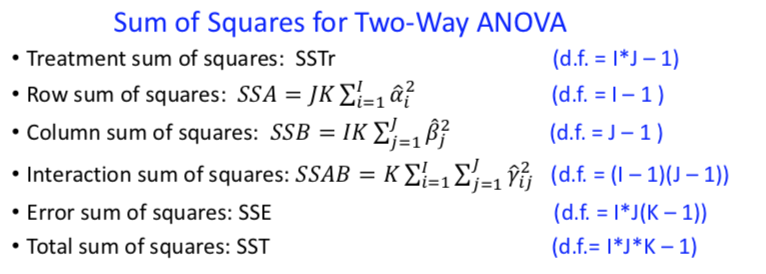
\includegraphics[width=.9\columnwidth]{degrees}

    There is a different statistic for each hypothesis

    \begin{equation*}
        F_{AB}^* = \frac{MSAB}{MSE} \qquad F_A ^* = \frac{MSA}{MSE} \qquad \frac{MSB}{MSE}
    \end{equation*}

    and

    \begin{equation*}
        MSA = \frac{SSA}{I - 1} \qquad MSB = \frac{SSB}{J - 1} \qquad MSAB + \frac{SSAB}{(I - 1)(J - 1)}
    \end{equation*}

    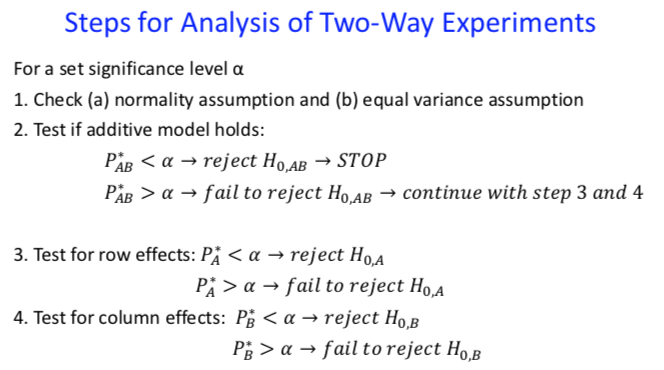
\includegraphics[width=\columnwidth]{steps-for-verification}

    \section{$2^p$ Factorial Experiment}
    \begin{itemize}
        \item $2^p$ factorial is a factorial experiment that has $p$ factors each of which has $2$ levels -- one level is designated ``high'' and the other is ``low''.
        \item
    \end{itemize}

    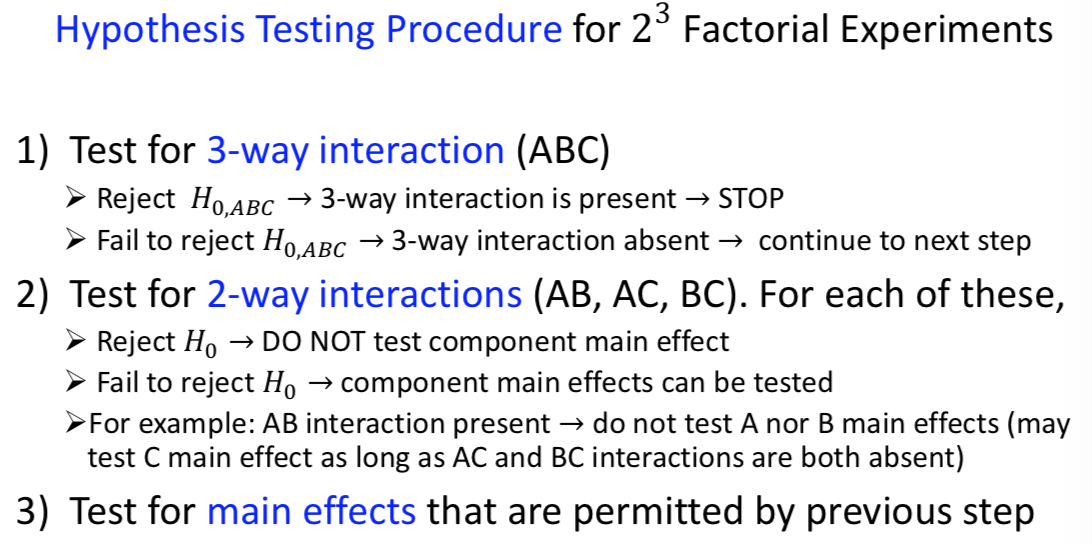
\includegraphics[width=\columnwidth]{factorial-expirement}

    \section{Bernoulli Distribution}
    The pmf is as follows

    \begin{equation*}
        p(x) = P(X = x) = \begin{cases}
            p & x = 1 \\
            1 - p & x = 0
        \end{cases}
    \end{equation*}

    \begin{itemize}
        \item Bernoulli's principle is as follows:
            \begin{itemize}
                \item $X = 1$ if the experiment results in ``success''
                \item $X = 0$ if the experiment results in ``failure''
            \end{itemize} \vspace{1mm}

        \item Notation $X \textasciitilde Benoulli(p)$
        \item With $X \textasciitilde Bernoulli(p)$, the mean and variance are as follows

            \begin{align*}
                \mu_x    &= p \\
                \sigma_x ^2 &= p(1 - p)
            \end{align*}
    \end{itemize}

    \section{Binomial Distribution}
    With $n$ trials, and same probability success rate $p$, and $X$ the number of successes in the $n$ trials

    \begin{equation*}
        p(x) = P(X = x) = \begin{cases}
            {n \choose x} p^x {(1 - p)}^{n - x} & x = 0, 1, \ldots, n \\
            0 & \text{otherwise}
        \end{cases}
    \end{equation*}

    where ${n \choose k} = \frac{n!}{k!(n - k)!}$

    \begin{itemize}
        \item The mean and variance of a binomial random variable is

            \begin{align*}
                \mu_x = np \\
                \sigma_x ^2 = np(1 - p)
            \end{align*}

        \item To estimate the success probability $p$ we can computer the sample proportion $\hat{p}$

            \begin{equation*}
                \hat{p} = \frac{\text{number of successes}}{\text{number of trials}} = \frac{X}{n}
            \end{equation*}

        \item The uncertainty of $\hat{p}$
            \begin{equation*}
                \sigma_{\hat{p}} = \sqrt{Var(\hat{p)}} \approx \sqrt{\frac{\hat{p}(1 - \hat{p})}{n}}
            \end{equation*}
    \end{itemize}

    \section{Poisson Distribution}
    The Poisson distribution arises frequently in scientific work. One way to think of the Poisson distribution is as an approximation to the binomial distribution when $n$ is large and $p$ is small.

    \begin{itemize}
        \item with $\lambda = np$, and notation $X \textasciitilde Poisson(\lambda)$

            \begin{equation*}
                p(x) = P(X = x) = \begin{cases}
                    \frac{e^{-\lambda}\lambda^x}{x!} & x = 0, 1, \ldots, n \\
                    0 & \text{otherwise}
                \end{cases}
            \end{equation*}

        \item The mean and variance are defined as follows

            \begin{equation*}
                \mu_x = \lambda \qquad \sigma_x ^2 = \lambda
            \end{equation*}
    \end{itemize}

    \section{The Normal Distribution}
    If a continuous random variable $x$ with mean $\mu$ and variance $\sigma^2$ has the following probability density function

    \begin{equation*}
        f(x) = \frac{1}{\sigma \sqrt{2\pi}} e^{-\frac{{(x - \mu)}^2}{2\sigma^2}}
        \end{equation*}

        The notation is $X \textasciitilde N(\mu, \sigma^2)$

        The standard unit equivalent

        \begin{equation*}
            Z = \frac{X - \mu}{\sigma}
        \end{equation*}

        \section{The Exponential Distribution}
        The notation is as follows $X \textasciitilde Exp(\lambda)$

        \begin{equation*}
            f(x) = \begin{cases}
                \lambda e^{-\lambda x} & x = 0, 1, \ldots, n \\
                0 & \text{otherwise}
            \end{cases}
        \end{equation*}


        \begin{itemize}
            \item The CDF of $X \textasciitilde exp(\lambda)$ is

                \begin{equation*}
                    F(x) = \begin{cases}
                        0 & x \leq 0 \\
                        1 - e^{-\lambda x} & x > 0
                    \end{cases}
                \end{equation*}

            \item The mean of $X \textasciitilde exp(\lambda)$ is $\mu_x = \frac{1}{\lambda}$

            \item The variance of $X \textasciitilde exp(\lambda)$ is $\sigma_x ^2 = \frac{1}{\lambda^2}$

            \item The exponential distribution is sometimes used to model the waiting time to an event. If events follow a Poisson process with rate parameter $\lambda$, and if $T$ represents the waiting time from any starting point until the next event, then $T \textasciitilde exp(\lambda)$.

            \item The lack of memory property is as follows: If $T \textasciitilde exp(\lambda)$, and $t$ and $s$ are positive number, then

                \begin{equation*}
                    P(T > t + s | T > s) = P(T > t)
                \end{equation*}
        \end{itemize}

        \begin{equation*}
            s_i ^2 = \sigma_i ^2 = \frac{1}{J_i - 1} \sum _{j = 1} ^{J_i} {\left( X_{ij} - \bar{X_{i.}} \right)}^2
        \end{equation*}

        Median time is

        \begin{equation*}
            \frac{\ln 2}{\lambda}
        \end{equation*}
    \end{multicols}
    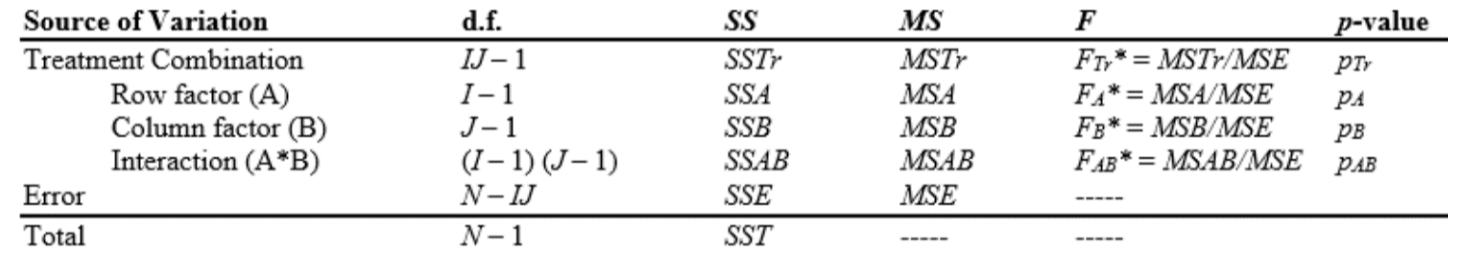
\includegraphics[width=\textwidth]{table}
\end{document}
